\documentclass[11pt,twoside]{article}

\usepackage{amsmath}
\usepackage{graphicx,epstopdf,epsfig}
\usepackage{amsmath,amssymb,amsbsy,bm}
%\usepackage[framed]{mcode}

\newlength{\toppush}
\setlength{\toppush}{2\headheight}
\addtolength{\toppush}{\headsep}

\renewcommand{\bottomfraction}{0.95}

\newcommand{\htitle}[3]{\begin{center}
\vspace*{-\toppush}
{\large MASSACHUSETTS INSTITUTE OF TECHNOLOGY}\\
{\small Department of Electrical Engineering and Computer Science}\\
\vspace*{1ex}{\Large #2}\end{center}
\noindent
\newline\parbox{6.5in}
{Fall 2013\hfill Issued : #1 \newline
 Problem Set 8 Solutions \hfill Due : #3\newline
%\profs \hfill %Handout #1\vspace*{-.5ex}\newline
%\mbox{}\hrulefill\mbox{}
}}

\newcommand{\mcO}{\mathcal{O}}
\newcommand{\handout}[3]{\thispagestyle{empty}
\pagestyle{myheadings}\htitle{#1}{#2}{#3}}

\setlength{\oddsidemargin}{0pt}
\setlength{\evensidemargin}{0pt}
\setlength{\textwidth}{6.5in}
\setlength{\topmargin}{0in}
\setlength{\textheight}{8.5in}


\newcommand{\pp}[2]{\frac{\partial #1}{\partial #2}}%
\newcommand{\ppp}[2]{\frac{\partial^2 #1}{\partial #2^2}}%
\newcommand{\dd}[2]{\frac{d #1}{d #2}}%
\newcommand{\ddd}[2]{\frac{d^2 #1}{d #2^2}}%
\newcommand{\matend}{\end{array}\right]}
\newcommand{\matc}{\left[\begin{array}{c}}
\newcommand{\matcc}{\left[\begin{array}{cc}}
\newcommand{\bb}{\mathbf{b}}
\newcommand{\bx}{\mathbf{x}}
\newcommand{\bA}{\mathbf{A}}
\newcommand{\DD}[2]{\frac{D #1}{D #2}}%
\newcommand{\Uvec}{\mathbf{U}}
\newcommand{\uvec}{\mathbf{u}}
\newcommand{\tauvec}{\bm{\tau}}
\newcommand{\omegavec}{\bm{\omega}}


\renewcommand{\Re}{\mathrm{Re}}


\begin{document}


\handout{Nov 19, 2013}{6.301 Solid State Circuits}{Nov 26, 2013}
\setlength{\parindent}{0pt}

\newcommand{\solution}{
 \medskip
 {\bf Solution:}
}

\hrulefill

\flushleft

\subsection*{Problem 1: Translinear Jungle Gym}
For each of the following circuits use the “Gilbert Principle”
to determine $I_o$ as a function of the other circuit variables.
All of these circuits simplify to simple expressions. \\
A differential output is denoted by an $I_o$ superimposed on an arrow,
 and double emitter arrows with $2A_E$ indicate that transistor has double the emitter area of the other transistors, thus its $I_S$ is twice as large. \\
Finally, use the method of open circuit time constants to estimate the $-3dB$ frequency for the circuit in part (a) only.
\vspace{8ex}
\begin{center}
\includegraphics[width=.9\textwidth]{trans1-soln}
\end{center}

\clearpage
\begin{center}
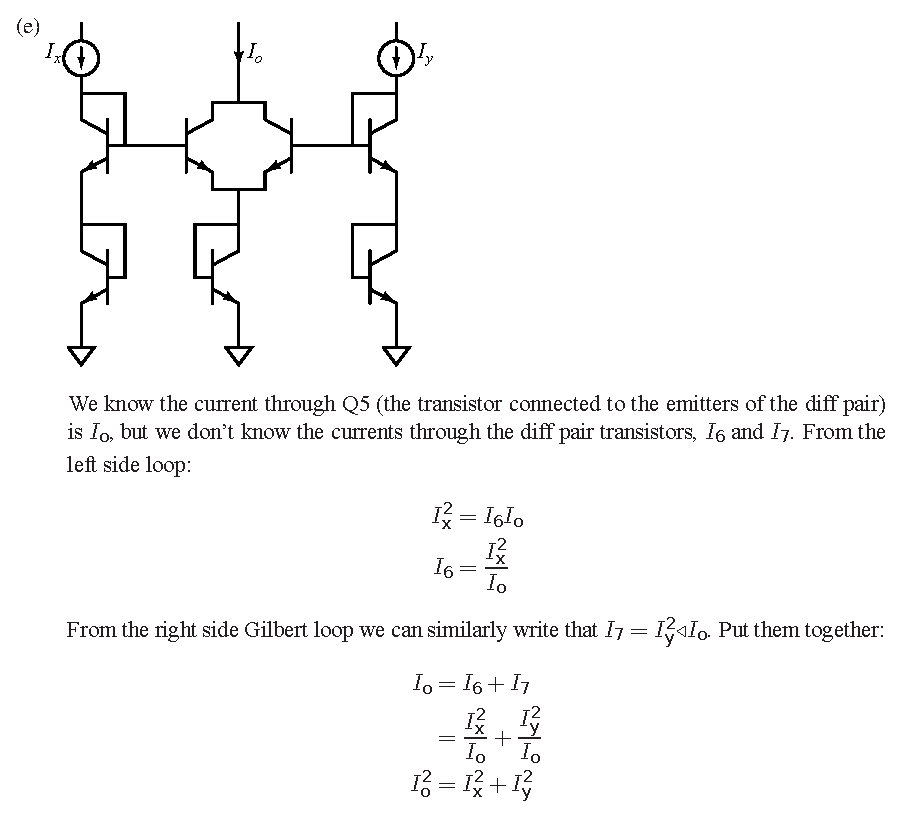
\includegraphics[width=.9\textwidth]{trans2-soln}
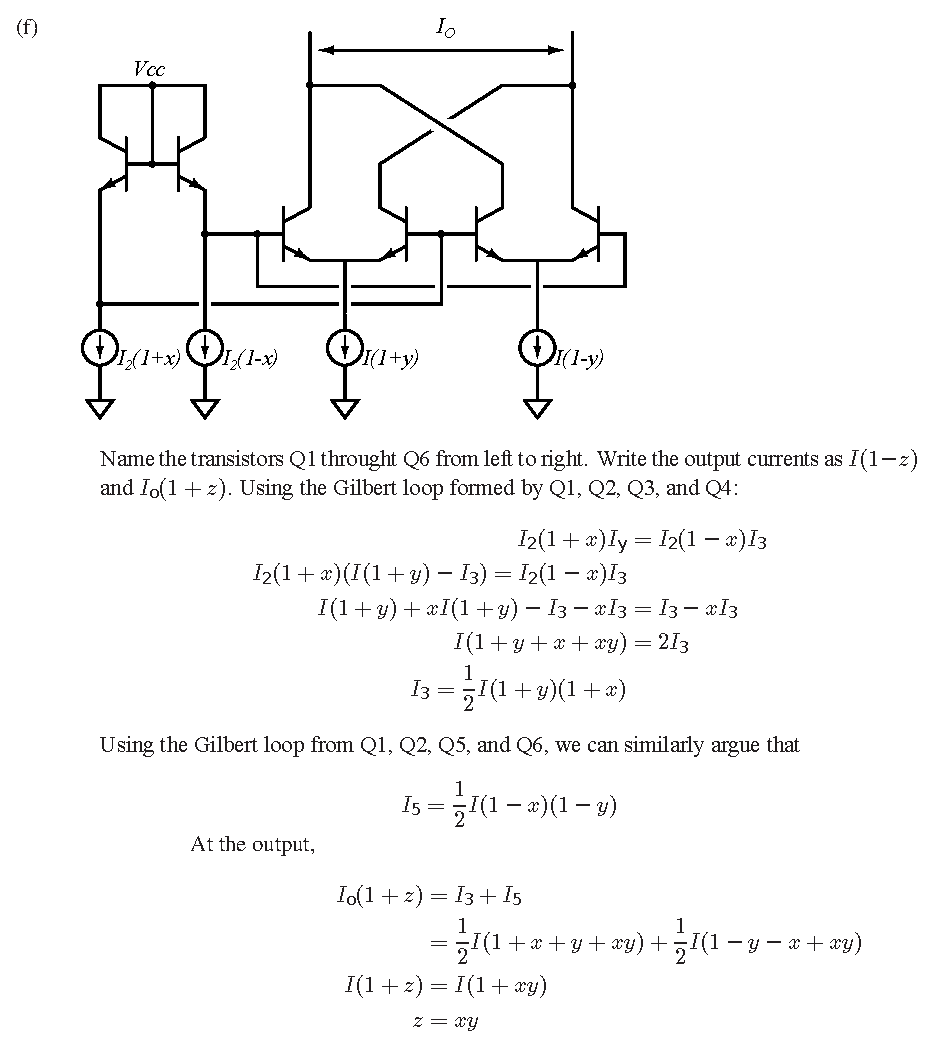
\includegraphics[width=.9\textwidth]{trans3-soln}
\end{center}
\clearpage
For the -3dB frequency of the circuit in part (a), assume the output node has some load impedance $R_L < r_o$.
This is reasonable because a current-source input load would look like $\frac{1}{gm}$ and a resistive load would likely be smaller than $r_o$.
For the worst-case OCT's, $R_\pi$ is $\frac{1}{gm}$ for all transistors.
For the diode-connected transistors, $R_\mu$ is 0 since the base is shorted to the collector.
The output transistor's $R_\mu = \frac{1}{gm}+{2R_o}$.
The middle transistor's $R_\mu = \frac{2}{gm}$.
\begin{align}
	\tau &= \frac{4C_\pi}{gm}+C_\mu(\frac{3}{gm}+2R_o) \\
	f_{-3dB} &= \frac{gm}{2\pi(4C_\pi+(3+2gmR_o)C_\mu)}
\end{align}
This circuit is {\it fast}.
\clearpage
\subsection*{Problem 2: Translinear Approximator}
Find $I_o=f(I_x)$, assuming well-matched transistors, negligible base currents, and $I_1=1A$.
Also assume $Q_A$ and $Q_B$ have emitter areas $24A_E$ and $2A_E$, respectively, while all other transistors have emitter area $A_E$. \\
What famous function does $I_o$ approximate for small $I_x$?\\
\vspace{4ex}
\begin{center}
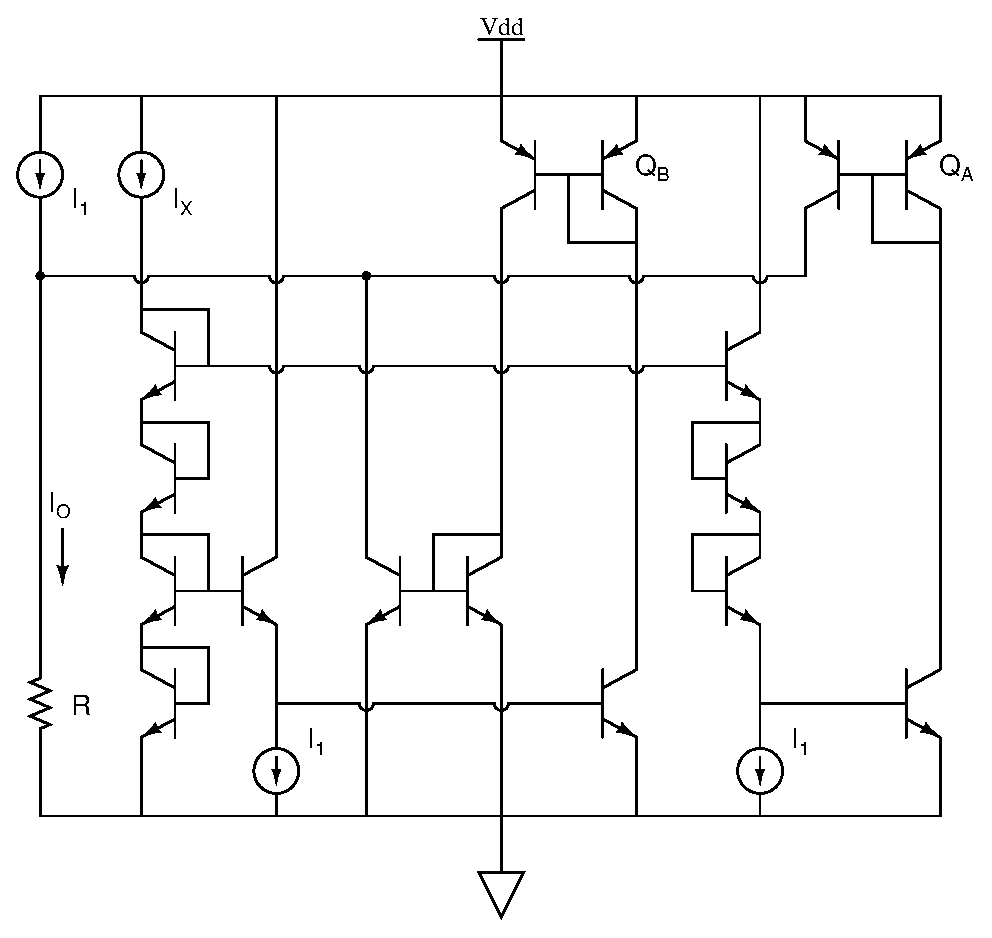
\includegraphics[width=.9\textwidth]{cos.eps}
\end{center}
\subsection*{Solution:}
Call the current through $Q_A$ and $Q_B$ $I_A$ and $I_B$, respectively.
The output current is:
\begin{align}
I_0&=I_1-\frac{I_A}{24}-\frac{I_B}{2}\\
\intertext{We can find $I_A$ from the Gilbert loop:}
I_x^4&=I_1^3I_A\nonumber \\
I_A&=\frac{I_x^4}{I_1^3}\nonumber \\
\intertext{and $I_B$:}
I_x^2&=I_iI_B\nonumber \\
I_B&=\frac{I_x^2}{I_1}\nonumber \\
\intertext{Substituting into (3)}
I_o &= I_1-\frac{I_x^2}{2I_1}+\frac{I_x^4}{24I_1^3}\\
\intertext{When $I_1=1$, (4) becomes:}
I_o &= 1-\frac{I_x^2}{2}+\frac{I_x^4}{24} \nonumber 
\end{align}
Which is the first two terms of the Taylor series expansion of cosine.

\subsection*{Problem 3: Base Current Error}
In the following circuit, assume $I_2=1mA$ and $\beta=100$.\\
\vspace{1ex}

\begin{center}
\includegraphics[width=.28\textwidth]{sqrtxy.eps}
\end{center}
\clearpage
\begin{enumerate}
	\item[(a)] Express $I_o$ in terms of $I_1$ and $I_2$.\\
 This is a simple Gilbert loop.
	\begin{align*}
	I_{c3}I_{c4}&=I_{c1}I_{c2}\\
	I_oI_o&=I_1I_2\\
	I_{o,ideal}&=sqrt{I_1I_2}
	\end{align*}
	\item[(b)] Assume we can tolerate a maximum $I_o$ error due to $\beta$ of 50\%.  For what range of $I_1$ is this circuit valid?
\vspace{1ex}
With finite $\beta$ we need to consider the effects of base current.
\begin{equation*}
I_{o,real} = sqrt{I_{c1}I_{c2}}
\end{equation*}
$I_{o,real}$ should never exceed $I_{o,ideal}$, so 
$\frac{\sqrt{I_{c1}I_{c2}}}{\sqrt{I_1I_2}}=\frac{1}{2}$ should have at least two solutions
which will provide the range of $I_1$.
\begin{equation}
I_{c1}+\frac{I_{c2}+I_o}{\beta}=I_1 \rightarrow 
I_{c1}=I_1-\frac{I_{c2}+\sqrt{I_{c1}I_{c2}}}{\beta}
\end{equation}
\begin{equation}
I_{c2} = (I_2-\frac{I_{c1}}{\beta})\frac{\beta}{\beta+1}
\end{equation}
Substituting equation (1) in to equation (2) gives:
\begin{equation*}
I_{c1}=I_1-(\frac{I_2}{\beta+1}-\frac{I_{c1}}{\beta(\beta+1)})-
\frac{\frac{\beta}{\beta+1}I_2I_{c1}-\frac{I_{c1}^2}{\beta+1}}{\beta}
\end{equation*}
Solve for $I_{c1}$ in terms of $I_1$ and $I_2=1$mA:
\begin{equation*}
I_{c1}=\frac{5050(\sqrt{-101(I_1^2-0.1I_1+987\times10^{-9})}+10099(I_1-9.9\times10^{-6}))}{50994951}
\end{equation*}
Solving $\frac{\sqrt{I_{c1}I_{c2}}}{\sqrt{I_1I_2}}=\frac{1}{2}$ for $I_1$:
\begin{equation*}
12.5\mu A < I_1 < 74.4mA
\end{equation*}
\end{enumerate}

\subsection*{Problem 4: Temperature Dependence and Compensation}
When we design a circuit, we prefer that it operate over a wide range of temperature.
Below is a voltage-biased current source with a temperature dependence heavily based on $R_E$ and $V_{be}$.
In the following circuit, assume that $\frac{1}{R} \frac{dR}{dT}=600ppm/^{\circ}C$ and $\frac{dV_{be}}{dT}=-2mV/^{\circ}C$. \\
\vspace{1ex}

\begin{center}
\includegraphics[width=.25\textwidth]{temp-dep.eps}
\end{center}

\begin{enumerate}
	\item[(a)] Find $\frac{dI_o}{dT}$.\\
\vspace{1ex}
Assume $I_B=0$.  Then $I_o=I_E=\frac{V_{BB}-V_{BE}}{R_E}$.
\begin{align*}
\frac{dI_o}{dT} &= \frac{d}{dT}(\frac{V_{BB}}{R_E})-\frac{d}{dT}(\frac{V_{BE}}{R_E})\\
 &= \frac{-V_{BB}\quad dR_E}{R_E^2 \quad dT}-\frac{R_E\frac{dV_{BE}}{dT}-V_{BE}\frac{dR_E}{dT}}{R_E^2}\\
 &= -\frac{V_{BB}}{R_E}(\frac{1}{R_E}\frac{dR_E}{dT})+
\frac{V_{BE}}{R_E}(\frac{1}{R_E}\frac{dR_E}{dT})-
\frac{1}{R_E}(\frac{dV_{BE}}{dT})\\
&= -I_o(\frac{1}{R_E}\frac{dR_E}{dT})-\frac{1}{R_E}(\frac{dV_{BE}}{dT})\\
\end{align*}

	\item[(b)] Find the value of $R_E$ in terms of $I_o$ that minimizes $\frac{dI_o}{dT}$.
\begin{align*}
\frac{dI_o}{dT} &= -I_o(\frac{1}{R_E}\frac{dR_E}{dT})-\frac{1}{R_E}(\frac{dV_{BE}}{dT})\\
&= -I_o(600\times10^{-6}/^{\circ} C)-\frac{1}{R_E}(-2\times10^{-3}V/^{\circ} C)\\
&\rightarrow R_{E_{min}}=\frac{3.33}{I_o}\\
\end{align*}
\end{enumerate}
\end{document}
